\begin{frame}{}
    \LARGE Advanced Diffusion Models: \textbf{Text-Conditioned}
\end{frame}

\begin{frame}[allowframebreaks]{Text-Conditioned Diffusion Models}
    \begin{figure}
        \centering
        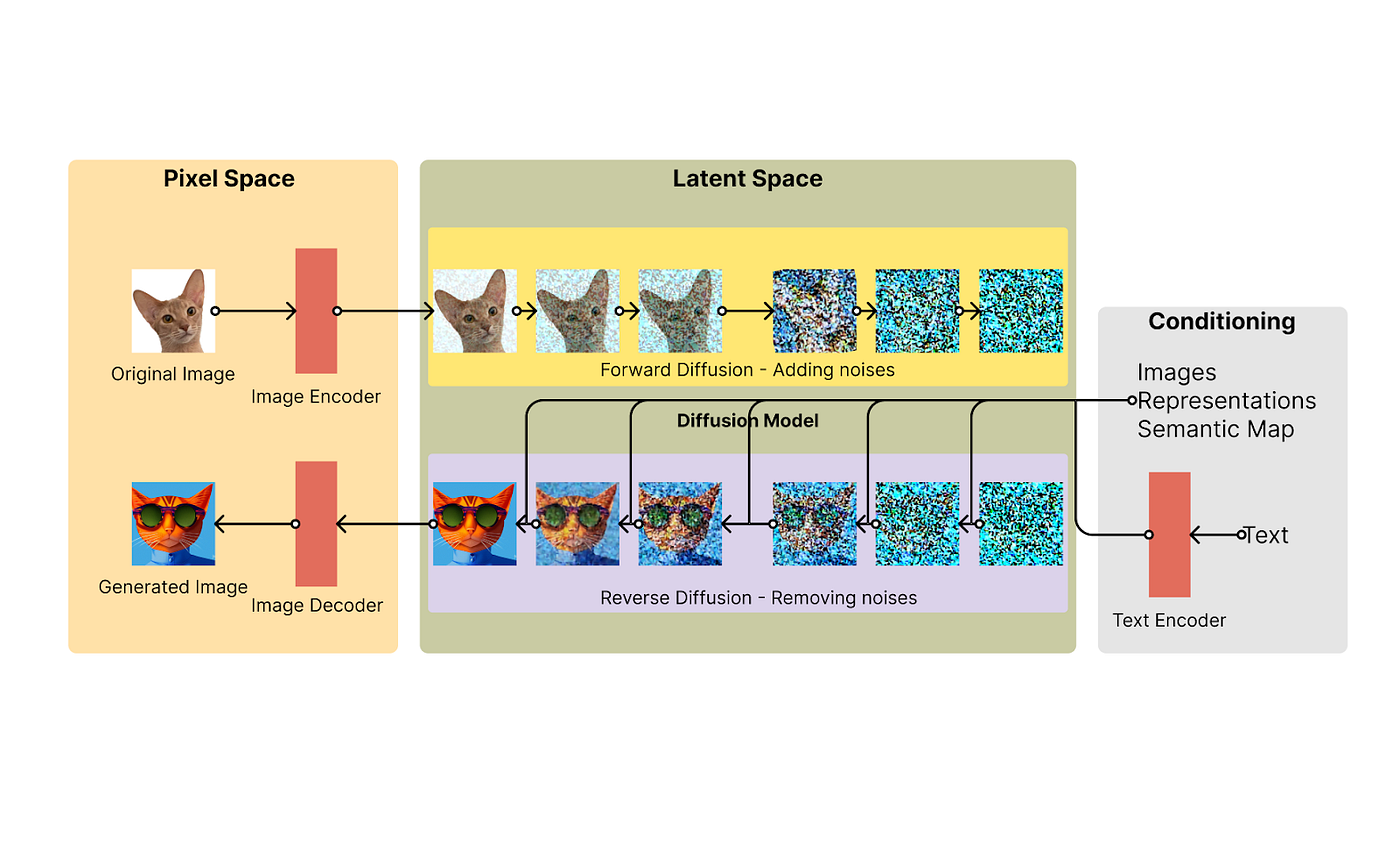
\includegraphics[width=1.05\linewidth,height=\textheight,keepaspectratio]{images/adv-img-gen/conditioning.png}
    \end{figure}
    \framebreak
\begin{itemize}
    \item \textbf{Overview:} Text-conditioned diffusion models enable the generation of highly specific images from textual prompts, such as \emph{"a cat wearing sunglasses standing in Times Square"}. These models leverage powerful text encoders, such as CLIP or transformer-based architectures, to extract semantic representations from the input text.

    \item \textbf{Diffusion Process:}
    \begin{itemize}
        \item Let $x_0$ denote the target image and $y$ the conditioning text.
        \item The diffusion process gradually adds noise to $x_0$ over $T$ steps, producing a sequence $\{x_t\}_{t=0}^T$.
        \item The reverse process aims to denoise $x_T \sim \mathcal{N}(0, I)$ back to $x_0$, conditioned on $y$.
    \end{itemize}

    \framebreak

    \item \textbf{Text Conditioning:}
    \begin{itemize}
        \item The text encoder maps $y$ to an embedding $e_y = \mathrm{TextEncoder}(y)$.
        \item This embedding is injected into the denoising UNet via cross-attention layers, allowing the model to align image features with the semantic content of the text.
    \end{itemize}

    \framebreak

    \item \textbf{Denoising Step:}
    \begin{itemize}
        \item At each denoising step $t$, the model predicts the noise $\epsilon_\theta(x_t, t, e_y)$:
        \[
        x_{t-1} = \frac{1}{\sqrt{\alpha_t}} \left( x_t - \frac{1-\alpha_t}{\sqrt{1-\bar{\alpha}_t}} \epsilon_\theta(x_t, t, e_y) \right) + \sigma_t z, \quad z \sim \mathcal{N}(0, I)
        \]
    \end{itemize}

    \framebreak

    \item \textbf{Training Objective:}
    \begin{itemize}
        \item The training objective is to minimize the difference between the true noise $\epsilon$ and the predicted noise:
        \[
        \mathcal{L}_{\text{diff}} = \mathbb{E}_{x_0, y, \epsilon, t} \left[ \left\| \epsilon - \epsilon_\theta(x_t, t, e_y) \right\|^2 \right]
        \]
    \end{itemize}

    \item \textbf{Effect of Conditioning:} By conditioning the denoising process on $e_y$, the model generates images that faithfully reflect the textual description. The cross-attention mechanism in the UNet ensures that relevant parts of the text influence corresponding regions in the image, enabling complex and coherent scene synthesis.
\end{itemize}
\end{frame}

\begin{frame}{Application: GLIDE - OpenAI}
\begin{figure}
    \centering
    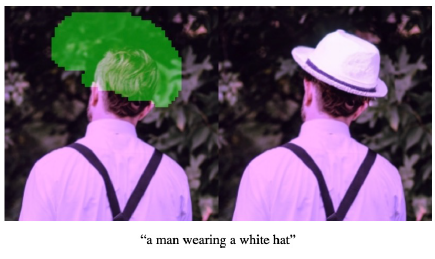
\includegraphics[height=0.8\textheight, width=\textwidth, keepaspectratio]{images/diffusion/diff_results_2.png}
    \caption*{Image Inpainting with GLIDE}
\end{figure}
\footnotetext{\href{https://arxiv.org/abs/2112.10741}{GLIDE: Towards Photorealistic Image Generation and Editing with Text-Guided Diffusion Models}}
\end{frame}
\begin{frame}{Application: DALL.E 2 - OpenAI}
\begin{figure}
    \centering
    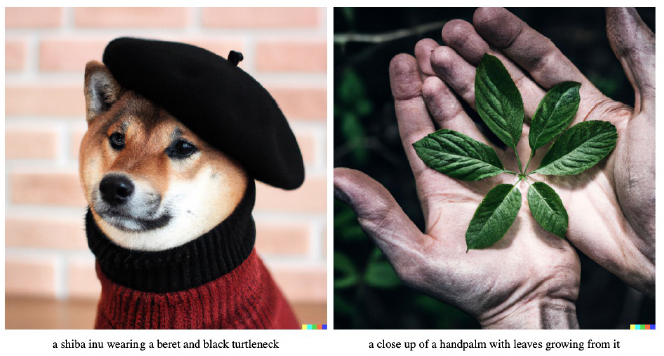
\includegraphics[height=0.8\textheight, width=\textwidth, keepaspectratio]{images/diffusion/diff_results_3.png}
    \caption*{Text to image generation eith DAll.E 2}
\end{figure}
\footnotetext{\href{https://arxiv.org/abs/2204.06125}{Hierarchical Text-Conditional Image Generation with CLIP Latents}}
\end{frame}

\begin{frame}{DALL.E 2 - OpenAI}
\begin{figure}
    \centering
    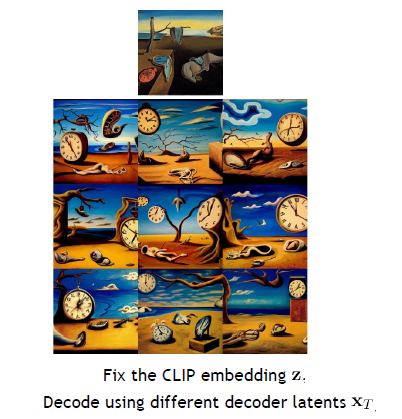
\includegraphics[height=0.8\textheight, width=\textwidth, keepaspectratio]{images/diffusion/diff_results_4.png}
    \caption*{Image Variations}
\end{figure}

\footnotetext{\href{https://arxiv.org/abs/2204.06125}{Hierarchical Text-Conditional Image Generation with CLIP Latents}}


\end{frame}

\begin{frame}{DALL.E 2 - OpenAI}
\begin{figure}
    \centering
    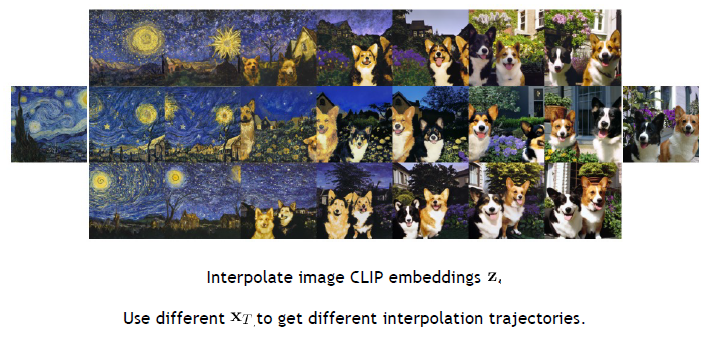
\includegraphics[height=0.8\textheight, width=\textwidth, keepaspectratio]{images/diffusion/diff_results_5.png}
    \caption*{Image interpolation}
\end{figure}

\footnotetext{\href{https://arxiv.org/abs/2204.06125}{Hierarchical Text-Conditional Image Generation with CLIP Latents}}

\end{frame}

\begin{frame}{DALL.E 2 - OpenAI}
\begin{figure}
    \centering
    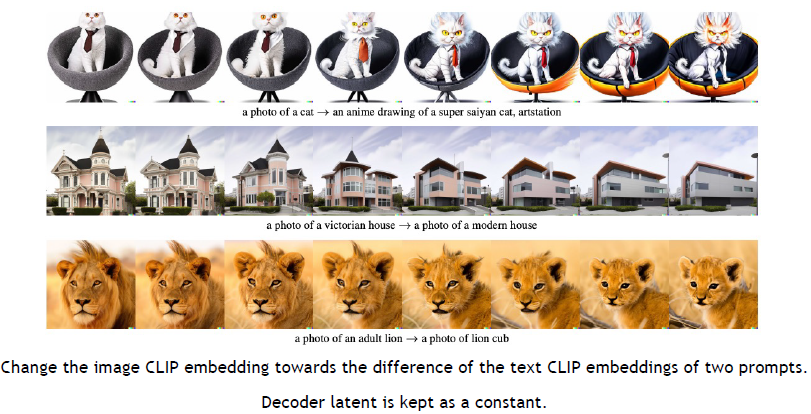
\includegraphics[height=0.8\textheight, width=\textwidth, keepaspectratio]{images/diffusion/diff_results_6.png}
    \caption*{Text Difference Image interpolation}
\end{figure}

\footnotetext{\href{https://arxiv.org/abs/2204.06125}{Hierarchical Text-Conditional Image Generation with CLIP Latents}}

\end{frame}
\begin{frame}{Imagen - Google}

\begin{figure}
    \centering
    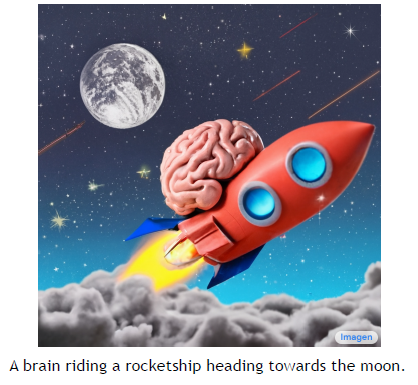
\includegraphics[height=0.8\textheight, width=\textwidth, keepaspectratio]{images/diffusion/diff_results_7.png}
\end{figure}

\footnotetext{\href{https://arxiv.org/abs/2205.11487}{Photorealistic Text-to-Image Diffusion Models with Deep Language Understanding}}
\end{frame}

\begin{frame}{Imagen - Google}

\begin{figure}
    \centering
    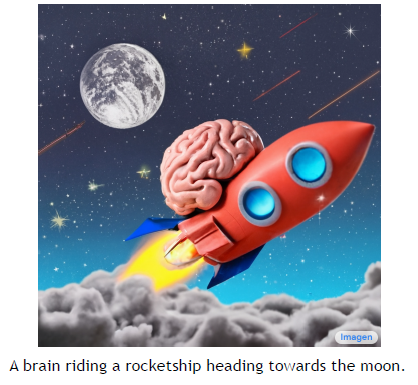
\includegraphics[height=0.8\textheight, width=\textwidth, keepaspectratio]{images/diffusion/diff_results_7.png}
\end{figure}

\footnotetext{\href{https://arxiv.org/abs/2205.11487}{Photorealistic Text-to-Image Diffusion Models with Deep Language Understanding}}
\end{frame}

\begin{frame}{Imagen - Google}

\begin{figure}
    \centering
    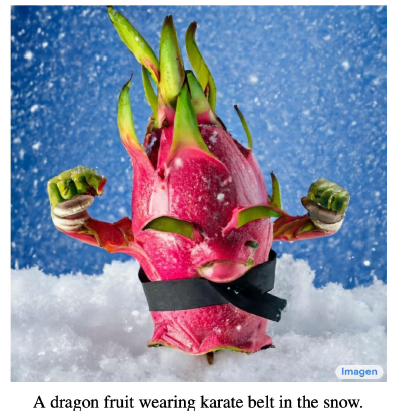
\includegraphics[height=0.8\textheight, width=\textwidth, keepaspectratio]{images/diffusion/diff_results_8.png}
\end{figure}

\footnotetext{\href{https://arxiv.org/abs/2205.11487}{Photorealistic Text-to-Image Diffusion Models with Deep Language Understanding}}
\end{frame}

\begin{frame}{Imagen - Google}

\begin{figure}
    \centering
    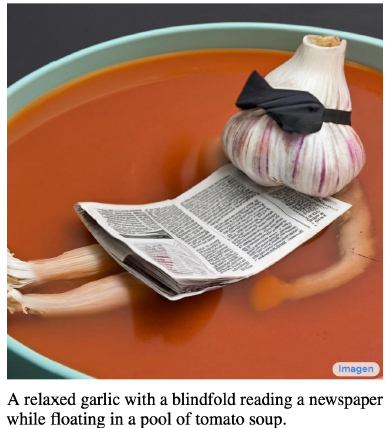
\includegraphics[height=0.8\textheight, width=\textwidth, keepaspectratio]{images/diffusion/diff_results_9.png}
\end{figure}

\footnotetext{\href{https://arxiv.org/abs/2205.11487}{Photorealistic Text-to-Image Diffusion Models with Deep Language Understanding}}
\end{frame}